\documentclass{standalone}
\usepackage{pgf-umlcd}
\begin{document}
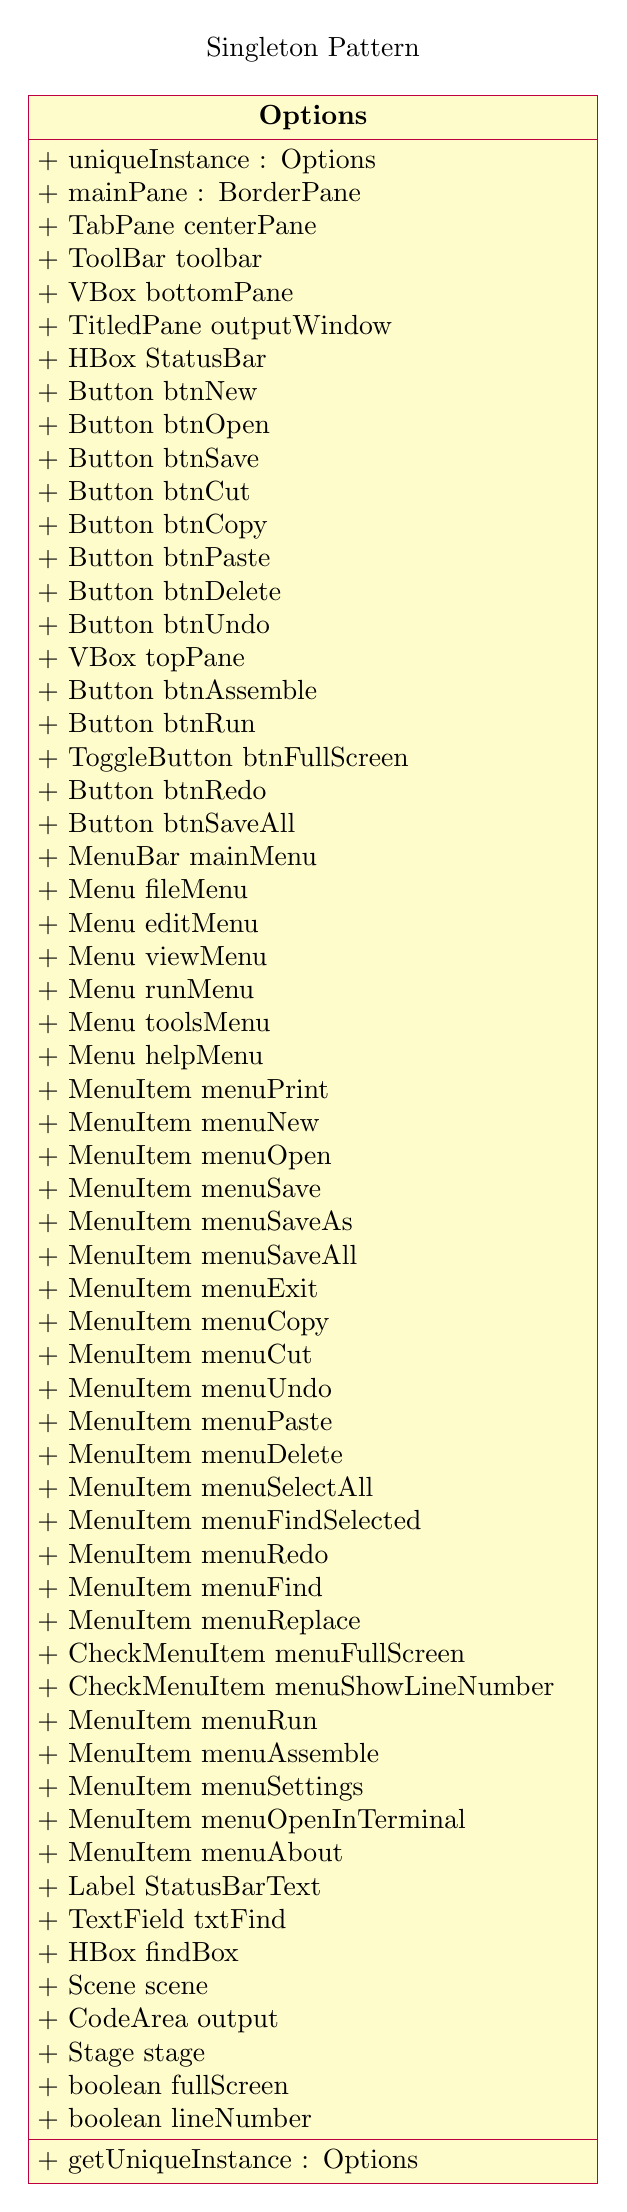
\begin{tikzpicture}
  \begin{class}[text width = 7cm]{Options}{0,0}
    \attribute{+ uniqueInstance : Options}
    \attribute{+ mainPane : BorderPane }
    \attribute{+ TabPane centerPane}
    \attribute{+ ToolBar toolbar}
    \attribute{+ VBox bottomPane}
    \attribute{+ TitledPane outputWindow}
    \attribute{+ HBox StatusBar}
    \attribute{+ Button btnNew}
    \attribute{+ Button btnOpen}
    \attribute{+ Button btnSave}
    \attribute{+ Button btnCut}
    \attribute{+ Button btnCopy}
    \attribute{+ Button btnPaste}
    \attribute{+ Button btnDelete}
    \attribute{+ Button btnUndo}
    \attribute{+ VBox topPane}
    \attribute{+ Button btnAssemble}
    \attribute{+ Button btnRun}
    \attribute{+ ToggleButton btnFullScreen}
    \attribute{+ Button btnRedo}
    \attribute{+ Button btnSaveAll}
    \attribute{+ MenuBar mainMenu}
    \attribute{+ Menu fileMenu}
    \attribute{+ Menu editMenu}
    \attribute{+ Menu viewMenu}
    \attribute{+ Menu runMenu}
    \attribute{+ Menu toolsMenu}
    \attribute{+ Menu helpMenu}
    \attribute{+ MenuItem menuPrint}
    \attribute{+ MenuItem menuNew}
    \attribute{+ MenuItem menuOpen}
    \attribute{+ MenuItem menuSave}
    \attribute{+ MenuItem menuSaveAs}
    \attribute{+ MenuItem menuSaveAll}
    \attribute{+ MenuItem menuExit}
    \attribute{+ MenuItem menuCopy}
    \attribute{+ MenuItem menuCut}
    \attribute{+ MenuItem menuUndo}
    \attribute{+ MenuItem menuPaste}
    \attribute{+ MenuItem menuDelete}
    \attribute{+ MenuItem menuSelectAll}
    \attribute{+ MenuItem menuFindSelected}
    \attribute{+ MenuItem menuRedo}
    \attribute{+ MenuItem menuFind}
    \attribute{+ MenuItem menuReplace}
    \attribute{+ CheckMenuItem menuFullScreen}
    \attribute{+ CheckMenuItem menuShowLineNumber}
    \attribute{+ MenuItem menuRun}
    \attribute{+ MenuItem menuAssemble}
    \attribute{+ MenuItem menuSettings}
    \attribute{+ MenuItem menuOpenInTerminal}
    \attribute{+ MenuItem menuAbout}
    \attribute{+ Label StatusBarText}
    \attribute{+ TextField txtFind}
    \attribute{+ HBox findBox}
    \attribute{+ Scene scene}
    \attribute{+ CodeArea output}
    \attribute{+ Stage stage}
    \attribute{+ boolean fullScreen}
    \attribute{+ boolean lineNumber}
    \operation{+ getUniqueInstance : Options}

  \end{class}
  \node [above=3mm] at (current bounding box.north) {Singleton Pattern};
\end{tikzpicture}
\end{document}
